\documentclass[a4paper, 12pt, oneside]{scrbook}
\usepackage[hyphens,spaces,obeyspaces]{url}
\usepackage[sorting = none, backend=bibtex]{biblatex}
\usepackage[english]{babel}
\usepackage[T1]{fontenc}
\usepackage[utf8]{inputenc}
\usepackage[hidelinks]{hyperref}
\usepackage{graphicx}
\usepackage{subcaption}
\usepackage{epstopdf}
\usepackage{lmodern}
\usepackage{float}
\usepackage{acronym}
\usepackage{booktabs}
\usepackage{caption}
\usepackage{csquotes}
\usepackage{enumitem}
\usepackage{fancyhdr}
\usepackage{url}
\usepackage{listings}
\usepackage[table]{xcolor}
\usepackage{wrapfig}
\usepackage{forest}
\usepackage{tabularx}
\usepackage{colortbl}
\usepackage{booktabs}
\usepackage[onehalfspacing]{setspace}
\usepackage{amsmath}
\usepackage{threeparttable}
\usepackage[english]{cleveref}
\renewcommand*{\headfont}{\normalfont}
\renewcommand*{\multicitedelim}{\addsemicolon\space}
\renewcommand*{\headrulewidth}{0pt}
\renewcommand*{\arraystretch}{1.5}
\setlength{\parskip}{1.5ex}
\makeatletter
% define new boolean conditional switch for whether
% the abstract is being typeset
\newif\ifabstract
% redefine `\chapter` so it only starts a new page if not typesetting
% the abstract; sets abstract conditional to false after doing so
\renewcommand\chapter{\ifabstract\relax\else%
	\if@openright\cleardoublepage\else\clearpage\fi%
	\fi
	\abstractfalse%
	\thispagestyle{plain}%
	\global\@topnum\z@
	\@afterindentfalse
	\secdef\@chapter\@schapter}

% command for putting the title and name above the abstract; switches
% abstact boolean to true for next `\chapter*` command...
\newcommand{\conclusion}{
	\if@openright\cleardoublepage\else\clearpage\fi
		\begin{center}
			\textbf{\larger{Summary}}\par
			\emph{Hier kommt nach der Fertigstellung der Arbeit noch eine Zusammenfassung der Arbeit mit ein oder mehreren Sätzen hin. Hier kommt nach der Fertigstellung der Arbeit noch eine Zusammenfassung der Arbeit mit ein oder mehreren Sätzen hin. Hier kommt nach der Fertigstellung der Arbeit noch eine Zusammenfassung der Arbeit mit ein oder mehreren Sätzen hin2. }\par
		\end{center}

	\abstracttrue}
\makeatother
\lstset
{
         basicstyle=\footnotesize\ttfamily,
         numbers=left,               	% Ort der Zeilennummern
         numberstyle=\tiny,          	% Stil der Zeilennummern
%         stepnumber=2,               	% Abstand zwischen den Zeilennummern
         numbersep=5pt,              	% Abstand der Nummern zum Text
         tabsize=2,                  	% Groesse von Tabs
         extendedchars=true,
         breaklines=true,            	% Zeilen werden Umgebrochen
         keywordstyle=\color{red},
            frame=b,
 %        keywordstyle=[1]\textbf,    	% Stil der Keywords
 %        keywordstyle=[2]\textbf,
 %        keywordstyle=[3]\textbf,
 %        keywordstyle=[4]\textbf, \sqrt{\sqrt{}}
         stringstyle=\color{white}\ttfamily,
         showspaces=false,
         showtabs=false,
         xleftmargin=27pt,
         framexleftmargin=27pt,
         framexrightmargin=5pt,
         framexbottommargin=4pt,
%         backgroundcolor=\color{lightgray},
         showstringspaces=false      	% Leerzeichen in Strings anzeigen ?
}
\addbibresource{bibliography.bib}

\begin{document}
	\frontmatter
	\def\doctype{T3\_3000}
\def\title{Grafana als (alternative) Dashboardlösung für industrielle „Use Cases“}
\def\author{Rico Kursidem}
\def\supervisor{Steffen Michalowski}

\begin{titlepage}

\vspace{10mm}

\begin{center}
	
	\vspace{5mm}
	\huge \title
	
	\vspace{34pt}
	\large \doctype
		
	\vspace{30pt}	
	\small Projekt für Angewandte Informatik \\
	\large Duale Hochschule Baden-Württemberg Mosbach \\
	\small Studienpartner \\
	\large AZO GmbH \& Co. KG \\
    \vspace{35pt}
    
    
\includegraphics[height=2.5cm]{prefix/image/logo-dhbw.eps}
    
\includegraphics[height=2.5cm]{prefix/image/logo-azo.png}
	
	\vspace{40pt}	
	\small von \\
	\large \author \\
	\small betreut von \\
	\large \supervisor
\end{center}

\vspace{75pt}


\vspace{49.7pt}

\fancypagestyle{empty}{
  \fancyhf{}
  \fancyfoot[C]{\today}
}

\end{titlepage}
	%\chapter*{Abbreviation} 
\begin{acronym}
	%A
	%B
	%C
	%D
	%E
	\acro{test}{Test}
	%F
	%G
	%H
	%I
	%J
	%K
	%L
	%M
	%N
	%O
	%P
	%Q
	%R
	%S
	%T
	%U
	%V
	%W
	%X
	%Y
	%Z
\end{acronym}
	\tableofcontents
	\listoffigures
	%\listoftables
	%\lstlistoflistings
	\nocite{*}

	\mainmatter

	\pagebreak
%	\conclusion
	\chapter{Einführung}
	%TODO Thema
	
	\noindent Daten und der Einsatz von ihnen im industriellen Umfeld ist nicht mehr wegzudenken. Die Fähigkeit, Daten visuell darzustellen und so dem Administrator des Systems Mustererkennung möglich zumachen, ist essentiell zur Entscheidungsfindung. Auch das Monitoring von Live-Daten ist wichtig. Diese Aufgaben übernehmen Dashboards auf denen Daten in verschiedensten Formen angezeigt werden können. Grafana ist eine Technologie mit der einfach und schnell Daten aus verschiedensten Datenquellen zusammengetragen und visuell dargestellt werden können. 
	
	\noindent Eine Eigene Lösung für die Auswertung von Daten zu entwickeln ist Zeitaufwendig und das Resultat vermisst viele Funktionen welche Stand der Technik sind. Deshalb soll Grafana als kostengünstige Alternative in Betracht gezogen werden. Es gibt mehrere Anforderungen an das System welche erfüllt werden müssen, darunter das Einbinden der vorhandenen Datenquellen und Erstellung von bereits existierenden Dashboards, welche in einem Fragenkatalog festgehalten wurden. Das Ziel dieser Arbeit ist es diesen Katalog zu beantworten und einen ersten Überblick zu liefern, ob Grafana als mögliches Visualisierungswerkzeug eingesetzt werden kann.
		
	\chapter{Technische Grundlagen}
	
		\section{Docker}
			\noindent Docker ist eine Open Source Virtualisierungssoftware mit welcher die Ausführung von Applikationen in Containern möglich ist. Jede Anwendung bekommt einen eigenen Container mit individueller Umgebung und läuft dann, parallel zu anderen Containern, auf dem selben Host. Dockercontainer sind leichtgewichtiger da sie sich, anders als VMs, ein gemeinsames Betriebssystem teilen. Außerdem werden redundante Dependencies von einzelnen Containern nicht dupliziert sondern als gemeinsame Ressource abgespeichert. Ein anderer Vorteil von Docker Containern ist der einfache Transport. In einem Image wird hierfür alle nötigen Informationen abgespeichert. Die Dependencies und der Code der Anwendung. Dann muss nur das Image übertragen, ein Container daraus erstellt und auf einem beliebigen Dockersystem gestartet werden und die Applikation läuft.
			
			\noindent Das Testsystem auf welches diese Arbeit basiert nutzt Docker zur bereitstellung zahlreicher Dienste. Wichtig für diese Arbeit sind der Grafana, Node-Red und Datenbank Container.
		\section{ACAS}
			\noindent ACAS ist eine intern bei AZO entwickelte Automatisierungsplattform. Sie soll eine Schnittstelle zwischen Bediener und Anlage sein. Dabei sollen diverse Aufgaben wie Virtualisierung, Fehlererkennung und Monitoring erfüllt werden. Grafana soll als Monitoringtool eingesetzt werden um Anlagen im Betrieb zu überwachen und Fehlerursachen frühzeitig zu erkennen um Schäden zu minimieren.
		\section{Grafana}
			\noindent Grafana ist eine Open Source Software mit der dynamische Dashboards zur Überwachung und Auswerten von Daten angefertigt werden können. Grafna bietet hierzu eine zugängliche und simple Benutzeroberfläche zur Erstellung von einzelnen Diagrammen die Panels genannt werden. Grafana bietet state of the Art funktionen wie da Verschieben und individualisieren von Oberflächen und zahlreiche Datenquellen, sodass es einen solide Lösung für Monitoring, Fehlererkennung und Analyse darstellt.
	
	\chapter{Funktionsanalyse}
	 
	 \section{Einbinden von Datenquellen}
	 
	 	\noindent In dem bereits bestehenden System, in welches Grafana integriert werden soll, liegen mehrere Datenquellen vor. Sichergestellt sollte der Import von Daten in Microsoft SQL Datenbanken und aus Rest APIs über Node-Red. Grafana unterstützt Microsoft SQL nativ als Datenquelle neben zahlreichen anderen Datenbanken. Die Dantenbank kann unter dem Menüpunkt Daten Sourcen eingebunden werden und es können weitere Einstellungen zur Authentifizierung gemacht werden. Um diese Datenquelle zu verwenden, können in den Panelen unter "Query" die Datenquelle ausgewählt und ein SQL Befehl abgesetzt werden um Daten anzuzeigen. In Abbildung \ref{fig:mssql_ein} ist der "Query" Reiter abgebildet mit einem SQL Befehl. 
	 	
	 	\begin{figure} [H]
	 		\centering
	 		\resizebox{\linewidth} {!} {
	 			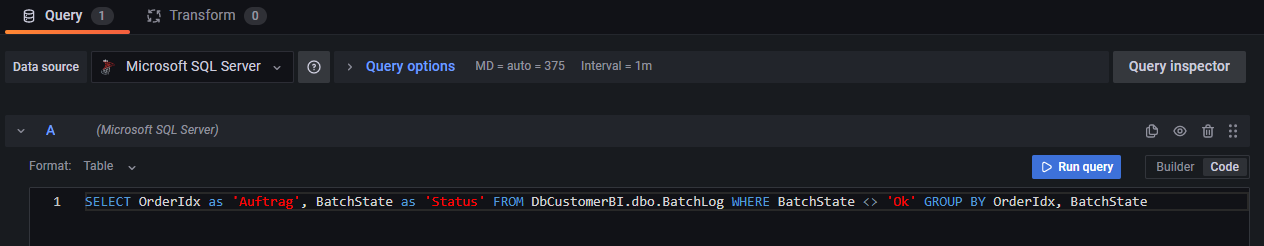
\includegraphics{res/mssql_einbinden.png}
	 			
	 		}
	 		\caption{Einbinden von MSSQL Datenbanken}
	 		\label{fig:mssql_ein}
	 	\end{figure}
 	
 		\noindent Die zweite Datenquelle welche als Anforderung an Grafana Eingebungen werden muss ist eine Node-Red Schnittstelle zu einem SPS-System. Hierbei sollen aktuelle Sensorwerte einer Anlage über eine Node-Red API abgerufen und in Grafana angezeigt werden. In Abbildung \ref{fig:nodered} ist der Node-Red Flow abgebildet, welcher Sensordaten aus einer SPS ausliest und als JSON an den Aufrufer der API zurückgibt. Die JSON besteht aus einem Array von Objekten mit vier Attributen. Name, Wert, Einheit und Farbe. Die Farbe kann als Statuswert genutzt werden, wobei beispielsweise ein zu kleiner Druck in Warnfarben angezeigt werden soll. 
 		
 		%TODO: Node-Red Flow Bild mit SPS als Quelle einfügen
 		%TODO: Beschreibung checken
 		
 		\begin{figure} [H]
 			\centering
 			\resizebox{\linewidth} {!} {
 				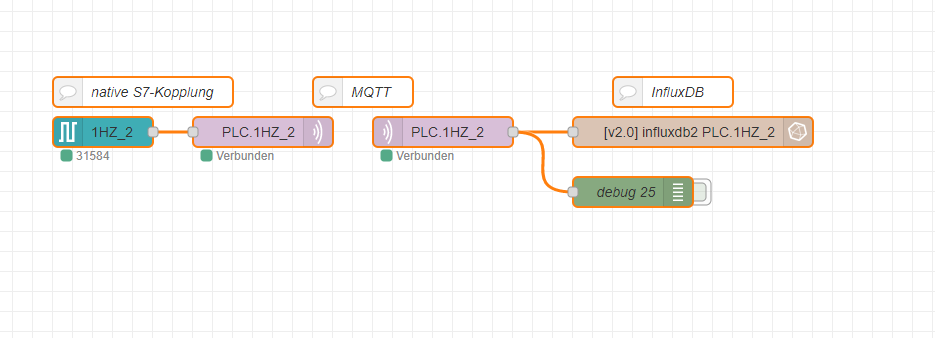
\includegraphics{res/nodered.png}
 				
 			}
 			\caption{Node-Red Flow mit Rückgabe einer JSON}
 			\label{fig:nodered}
 		\end{figure}
 	
	 	\noindent Um JSON Daten in Grafan verarbeiten zu können muss ein Plugin integriert werden. Hierbei fiel die Entscheidung auf das "Infinity" Plugin von Sriramajeyam Sugumaran da es neben der Integration von JSON Daten auch XML, CSV und weitere Datenformate unterstützt und regelmäßige Updates bekommt. In den Data Sourcen Einstellungen können weitere Einstellungen vorgenommen werden, die für den in dieser Arbeit nicht von Nöten sind. Wird die Data Source in einem Panel dann ausgewählt, muss die Adresse des API Aufrufs und optionale Übergabe Parameter eingetragen werden. Bei jeder Aktualisierung wird der API Abfrage getätigt und die Daten visualisiert. 
	 	
	 	\noindent Um die Sensordaten ansehnlich zu präsentiere, können Transformationen genutzt werden. Im Transformationen Reiter kann die Funktion "Rows from Fields" wie in Abbildung \ref{fig:transformation} ausgewählt werden, welche die Werte gewisser Spalten zu Konfigurationswerten übernimmt. 
	 	
	 	\begin{figure} [H]
	 		\centering
	 		\resizebox{75mm} {!} {
	 			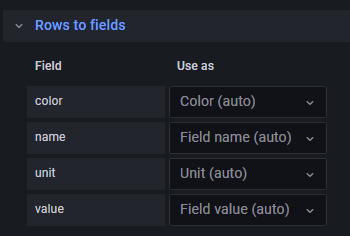
\includegraphics{res/transformation.png}
	 			
	 		}
	 		\caption{Transformation der Sensordaten}
	 		\label{fig:transformation}
	 	\end{figure}
 		
	 \section{Interaktion zwischen Grafen}
	 	
	 	\subsection{Filterungen durch Variablen}
	 	
	 	\noindent Grafana bietet dashboardweite Variablen, welche zuvor festgelegte Werte annehmen können. Diese Werte sind entweder manuell Eingetragen oder aus Datenquellen ausgelesen. In den Dshboardeinstellungen können Variablen angelegt und ihre Wertauswahl konfiguriert werden. Jede Variable kann ganz oben auf einem Dashboard angezeigt und dort anhand eines Drop-Down-Menüs gesetzt werden. 
	 	
	 	\noindent 
	  	
		\subsection{Links}
		 
			\noindent Bei Verlinkungen werden zwischen drei verschiedenen Links unterschieden. Dashboard Links, Panel Links und Data Links. Dashboardlinks können in den Dashboardeinstellungen erstellt werden und erscheinen dann in der oberen rechten Ecke des Dashboards. Um einen Link des Zieldashboards zu erstellen muss auf das Teilensymbol 
\includegraphics{res/teilensymbol.png} neben dem Namen geklickt werden und der Link kopiert werden. Panel Links sind Verlinkungen, welche an einem Panel angehangen sind. Sie erscheinen in der oberen linken Ecke eines Panels. Data Links können innerhalb eines Panels angelegt werden und können auf Informationen zugreifen, welche Daten in der Grafik gedrückt wurden. 
			 
			\noindent Um Informationen von einem Dashboard zum nächsten zu übermitteln können die Dashboardweiten Variablen verwendet werden. In Tabelle \ref{tab:links} ist der Syntax der verschiedenen Übergabemöglichkeiten aufgeführt. Es können konstante Werte, Dashboardvariablen oder Datenpunkte übergeben werden wobei bei der Eingabe von einem Dollarzeichen Grafana bereits alle möglichen Felder in einem Drop-Down-Menü vorschlägt und bei Auswahl den korrekten Syntax einträgt. \texttt{varName} ist dabei die Variable des Zieldashboards welche den gewählten wert annehmen soll.
			 
			\begin{figure} [H]
				\centering
				\resizebox{\linewidth} {!} {
			 		\begin{tabular}[h]{|l|c|}
			 			\hline
			 			Variable & Übergabe im Link \\
			 			\hline
			 			Konstante & \texttt{var-varName=value} \\
			 			\hline
			 			Variable &  \texttt{var-varName=\${DashBoardVar}} \\
			 			\hline
			 			Datenpunkt &  \texttt{var-varNname=\${\_\_data.fields.FieldName}} \\
			 			\hline
			 			Zeitintervall als url &  \texttt{\${\_\_url\_time\_range}} \\
			 			Intervall Start& \texttt{\$\_\_timeTo()} \\
			 			Intervall Ende& \texttt{\$\_\_timeFrom()} \\
			 			\hline
			 		\end{tabular}
		 		}
		 		
			 	\caption{Übergabeparameter in Links}
			 	\label{tab:links}
			\end{figure}
		 
		 	\noindent es kann auch auf das selbe Dashboard verlinkt und die Variablen gesetzt werden, woduch die manipulation von Panelen über den Klick auf ein anderes Panel ermöglicht wird.
			 
			 
		\subsection{Annotationen}
			 
			\noindent Annotationen können genutzt werden um bestimmte Ereignisse aus Zeitreihen auf dem gesamten Dashboard hervorzuheben. Diese Ereignisse können durch eine Datenquelle als Zeitabhängige Datenpunkte eingelesen werden. Sie werden dann auf jedem Zeitreihen Grafen markiert wie in Abbildung \ref{fig:annotations} die Fehlermeldungen in rot.
			 
			 \begin{figure} [H]
			 	\centering
			 	\resizebox{\linewidth} {!} {
			 		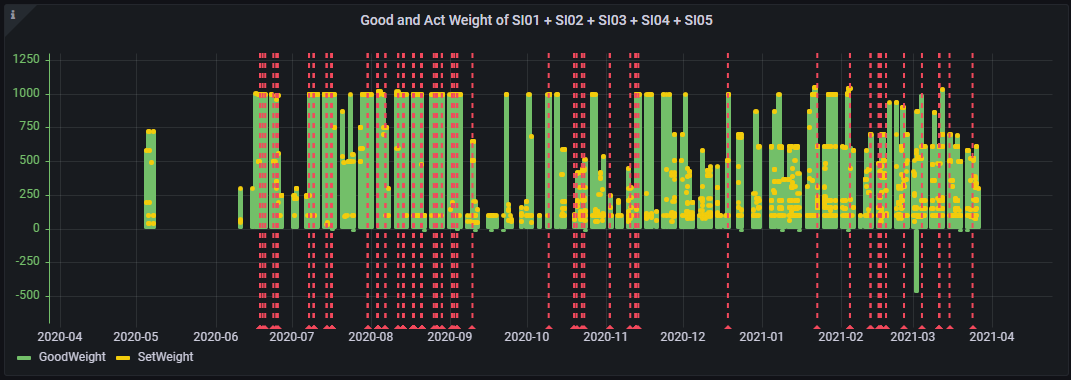
\includegraphics{res/annotaitons.png}
			 		
			 	}
			 	\caption{Annotationen in einer Zeitreihe}
			 	\label{fig:annotations}
			 \end{figure}
	 
	 \section{Berechtigungen und Rollenkonzepte}
	 \section{Erscheinungsbild und Design}
	 % Eher auf Fragen eingehen
	
	\frontmatter
	\printbibliography

\end{document}
